\section{Performance}
As could be seen in section \ref{approaches}, there are numerous ways to compute semantics of abstract argumentations. Furthermore, each approach can be implemented using different algorithms, programming languages or existing systems. With such a range of possibilities it is important to reflect on the existing solvers.

Results of ICCMA 2017 competition \citep{iccmaResults} gives an interesting overview of existing solvers and their performance. As shown in the table \ref{table:iccmaResultsbySolver}, majority of the winning solvers have been implemented using SAT based approach, and only winner of Stage semantic track has been implemented using CSP based approach. 

Furthermore, majority of the solvers were using reduction based approaches, where computing semantics have been reduced to different, well defined problems. Out of overall 16 solvers submitted to ICCMA 2017 (appendix \ref{appendix:ICCMASubmissions}), only three of them were using a direct approach - labeling based approach. Although none of those solvers won any track, based on the figure \ref{fig:coTrack} to figure \ref{fig:prTrack}, it can be seen that their overall performance was mediocre. The average time on computing various semantics and tasks could be as high as double that of the winning solvers. Furthermore, the scores accumulated by those solvers were significantly smaller than for the winning solvers, especially for Semi-Stable (figure \ref{fig:ssTrack}) and Stage Track (figure \ref{fig:stTrack}).


\subsection{Scalability}
Based on the results from ICCMA 2017 competition it could be seen that majority of the solvers producing correct solutions, based on the overall scores, have a relatively low execution time. The size of benchmark argumentation frameworks range from small frameworks of up to twenty to thousands of arguments and attacks.

Each task in the track contained 350 different argumentation frameworks. Defining difficulties of benchmark argumentation frameworks and selecting individual frameworks for the competition have been done using solvers from ICCMA 2015 competition. Number of representative solvers have been selected and ran for each group of benchmark frameworks. Table \ref{table:iccmaCategories} shows the selected categories and number of argumentation frameworks in each of them \citep{results_sildes}.

\renewcommand{\arraystretch}{1.5}
\begin{table}
	\caption{ICCMA 2017 benchmark frameworks categories}
	\label{table:iccmaCategories}
	\centering
	\[\tabulinesep = 3mm
	\begin{tabu}{p{0.2\textwidth} p{0.2\textwidth} p{0.5\textwidth}} 
		\toprule
		\textbf{Category } & \textbf{Count } & \textbf{Definition }                                                        \\ 
		\hline \hline
		Very Easy          & 50              & Instances solved by all representative solvers in less than 6 seconds  \\ \hline
		Easy               & 50              & Instances solved by all representative solvers in less than 60 seconds      \\ \hline
		Medium             & 100             & Instances solved by all representative solvers within 10 minutes            \\ \hline
		Hard               & 100             & Instances solved by at least one representative solver within 1200 seconds  \\ \hline
		Too Hard           & 50              & Not solved by representative solvers within 1200 seconds                    \\ \hline
		\bottomrule
	\end{tabu}
	\]
\end{table}

Most of the tracks for each extension consist of four individual tasks. Hence, with 350 argumentation frameworks selected for each task and 1 point being assigned for each correct result, the maximum score per semantic is 1,400, with the exception of Stage and Ideal extension, where maximum is 700 points (only two tasks per extension). 

\begin{landscape}
	\begin{figure}
		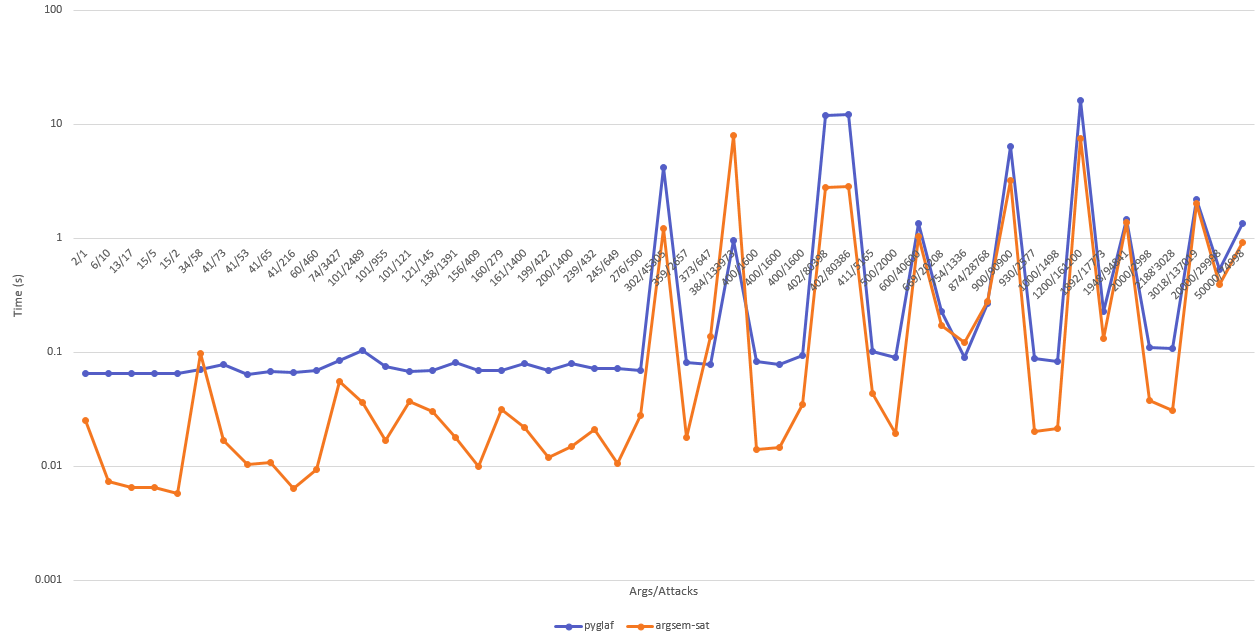
\includegraphics[width=21cm]{pyglaf_argsemsat}
		\caption{Pyglaf and argsem-sat timing results for Stable extension}
		\label{fig:pyglafArgsemsat}
	\end{figure}
\end{landscape}

Based on figures \ref{fig:coTrack} to \ref{fig:prTrack}, it can be seen that at least half of the solvers scored over 1,000 points for complete, stable, semi-stable and preferred extensions. This indicates that majority of the solvers submitted to ICCMA 2017 can easily manage large and complex argumentation frameworks, hence they do scale appropriately. Of course there are some limitations in terms of performance on the massive frameworks, thus no solver received maximum points for any of the semantics. 

Figure \ref{fig:pyglafArgsemsat} shows the chart of execution times of two winning solvers: Pyglaf and argsem-sat, for computing all stable extension from the provided benchmark argumentation frameworks. As it can be seen, execution time for both solvers is consistent for frameworks up to 300 arguments. Beyond that, there are some instances where it took the solvers significantly longer to compute the extensions, but no longer then 16 seconds in any of those cases. Even for the argumentation framework with 50,000 arguments and 74,998 attacks it took each of the solver around 1 second to produce the results. 

However, there are number of solvers with small number of overall points and/or high mean execution time. For example, ArgTools \citep{argtools} scored relatively low, close to zero, in Stage and Semi-Stable extensions, and argmat-clpb for Complete and Stable with high mean execution time. 

Although the solvers and results are only taken from the ICCMA 2017 competition, it indicates that a number of solvers exists, that are able to compute extensions efficiently. Furthermore, they can easily scale to cope with massive argumentation frameworks. 